\documentclass[10pt,twocolumn]{article}

\usepackage[a4paper,margin=2.1cm]{geometry}
\usepackage[utf8]{inputenc}
\usepackage[T1]{fontenc}
\usepackage{times}
\usepackage{graphicx}
\usepackage{booktabs}
\usepackage{amsmath}
\usepackage{url}
\usepackage[hidelinks]{hyperref}
\usepackage{caption}
\captionsetup{font=small,labelfont=bf}

\title{\vspace{-1.2cm}\bfseries SIV: Semantic Ifs over Images\\
\large Logit-Readout Decisions with a Vision--Language Model}

\author{%
Samuel Otero Agraso\\
\small\url{https://github.com/XxSamaxX/siv-semantic-if-vision}
}
\date{}

\begin{document}
\maketitle

\begin{abstract}
\noindent
Recent open implementations read a decision directly from a language model's
answer-token logits instead of decoding text, turning a model into a
runtime-defined conditional---a \emph{semantic if}. We port this readout
unchanged to a vision--language model and evaluate it on MMBench
(en/dev, 4329 items) plus a small hand-built probe. Qwen3-VL-4B reaches
87.4\% with one forward pass per item at 91\,ms, and 82.2\% under MMBench's
CircularEval protocol, which rotates the answer options.

Our main results concern the confidence signal rather than the score. The
softmax over answer slots, which these systems report as a probability, is
$\geq 0.99$ on 52\% of the model's own errors: it claims near-certainty on more
than half of what it gets wrong. The logit gap behind that same number predicts
correctness with AUC 0.894 and supports a usable operating point---thresholding
at 16 nats answers 66\% of items at 98.4\% accuracy, against an 87.4\% base
rate. The gap also predicts order sensitivity almost perfectly (AUC 0.980):
rotating options changes the winner on 11.7\% of items, and those items have a
median gap of 2.7 nats against 22.8 for the stable ones, which bounds when
order calibration is worth its $n$ forward passes.

Two negative results survive the scale-up. First, difficulty is not
epistemics: on 12 normative questions no model can ground, the gap
distribution shifts (median 8.8 vs 20.9 nats, AUC 0.788, $p=0.006$) but
overlaps so heavily that the best threshold still admits 7 of 12---the model
asserts that a photograph requires legal consent at 15.6 nats, as confidently
as it reports that no dog is present at 26.4. Second, our own 22-item probe
scored 22/22 with every softmax probability above $0.9993$, which we initially
read as universal saturation; the 4329-item run shows that this was a property
of an over-easy benchmark, and we report it as a caution about small
author-written test sets.
\end{abstract}

\section{Introduction}

A recurring pattern in recent agent tooling is to stop asking a language model
for text and ask it for a decision. The construction is simple: phrase the
decision as a lettered multiple choice, run a single forward pass, and read the
logits at the final position restricted to the tokens \texttt{A}, \texttt{B},
\texttt{C}. There is no decoding loop, so the cost is one prefill. The open
SemIf project \cite{semif} publishes this readout as a baseline, and the
JEV-CPU port \cite{jevcpu} demonstrates it on a laptop CPU with a 0.6B model.
Practitioners describe the result as a \emph{semantic if}: a conditional whose
predicate is written in natural language at runtime rather than compiled.

The attraction for computer vision is immediate. A detector trained on a fixed
label set answers ``is there a person'' but cannot answer ``is this photograph
posed'', ``is the white balance wrong'', or ``is the meal already in progress''.
These are not classes; they are predicates. If the readout transfers to a
vision--language model, the predicate becomes free text and no training set is
required.

This paper reports what happens when it does transfer. Our contributions are:

\begin{enumerate}\itemsep2pt
\item A port of the readout to a vision--language model in which the scoring
      path is byte-identical to the text implementation; only prompt
      construction and model loading differ (Section~\ref{sec:method}).
\item An evaluation on MMBench en/dev: 87.4\% at 91\,ms per item, 82.2\% under
      CircularEval (Section~\ref{sec:mmbench}), plus a 22-item adversarial
      probe the model answers in full (Section~\ref{sec:accuracy}).
\item The reported probability is not merely miscalibrated but actively
      misleading: it exceeds 0.99 on 52\% of the model's errors. The logit gap
      behind it predicts correctness with AUC 0.894 and supports abstention at
      98.4\% accuracy over 66\% of items (Sections~\ref{sec:saturation}
      and~\ref{sec:mmbench}).
\item A characterisation of position bias: 1--2 nats in magnitude, flipping the
      winner on 11.7\% of items, with the gap predicting order-stability at
      AUC 0.980. This bounds when order calibration earns its $n$ forward
      passes (Section~\ref{sec:order}).
\item A negative result we consider the most consequential for deployment: the
      gap does not separate answerable perceptual questions from ungroundable
      normative ones well enough to gate them (Section~\ref{sec:families}).
\item A methodological caution, learned the hard way: our own 22-item benchmark
      reported universal softmax saturation and zero order sensitivity, and the
      4329-item run refuted both.
\end{enumerate}

\section{Related work}

Open-vocabulary detection attacks the same limitation from the other side.
CLIP-style image--text alignment \cite{radford2021clip} underpins detectors
such as OWL-ViT \cite{minderer2022owlvit}, Grounding DINO
\cite{liu2023groundingdino} and YOLO-World \cite{cheng2024yoloworld}, which
accept a free-text vocabulary and localise its members. These systems remain
far faster than a vision--language forward pass and they return boxes, which
the readout studied here does not. They are, however, restricted to naming
things: they cannot evaluate a predicate over a scene. The two approaches are
complementary rather than competing, and a natural composition is to let a
detector propose regions and a semantic if evaluate predicates on the crops.

Our negative results connect to two literatures. Position bias in multiple
choice prompting is well documented \cite{zheng2024mcq}, and contextual
calibration \cite{zhao2021calibrate} is the standard remedy; we measure the
bias in nats and find it an order of magnitude smaller than the decision
margins on perceptual items, which bounds when that remedy is worth its cost.
Separately, modern networks are known to be poorly calibrated
\cite{guo2017calibration}; we show a sharper failure specific to this readout,
where the reported probability is not merely miscalibrated but constant.
Finally, object hallucination benchmarks such as POPE \cite{li2023pope}
establish that vision--language models assert the presence of absent objects;
our false-premise and absence items probe the same behaviour and, notably, do
not reproduce it at this model scale.

\section{Materials and methods}
\label{sec:method}

\subsection{The decision readout}

A decision is a tuple of evidence, a criterion, and 2--16 options. The prompt
is a JSON payload naming each option with a letter, under a system instruction
to answer with that letter alone. The implementation verifies that each letter
encodes to exactly one token with an exact decode round trip, and that
appending the letter does not alter the tokenisation of the prompt that
precedes it; both checks raise rather than silently degrade. A single forward
pass with \texttt{use\_cache=False} yields the final-position logit vector,
which is indexed at the answer-slot tokens. A softmax over those few entries
produces the reported probabilities.

\subsection{Extension to images}

We changed exactly two things. The user turn carries an image part before the
JSON payload, and the model is loaded as an image-text-to-text model in
bfloat16 on the GPU. The slot verification, the forward call and the logit
indexing are unchanged from the text implementation, so results are directly
comparable. At the processor's default resolution a $640\times480$ photograph
expands to roughly 300 visual tokens, giving prompts of 351--413 tokens in our
benchmark.

\subsection{Benchmark}

We wrote 22 decisions over four photographs from COCO \emph{val2017}. Twelve
are ordinary perceptual judgements, three of which a fixed-vocabulary detector
could also answer and act as controls. Ten target families known to be
difficult for vision--language models: exact counting, absence, a false-premise
question (the colour of a car in an image containing no car), an unanswerable
question (the time of day in a windowless interior), fine-grained comparison,
and spatial relation. Ground truth was written by the author from the images.
One label was initially wrong---we judged a brand mark illegible, and the model
read it correctly---and was corrected after visual inspection of an enlarged
crop; we report this because the corrected item is the hardest in the set.

A second set of 12 \emph{normative} questions was written to be structurally
identical but institutionally ungrounded: whether consent must be obtained,
whether a retention policy requires deletion, whether a model release has
expired. Each carries one sentence of evidence and two options. No model can
answer these from the evidence given, because the answer depends on a policy
it has never seen.

\subsection{Order calibration and the logit gap}

For each decision we optionally re-score under all cyclic rotations of the
option list and average in logit space. We record, per decision, the gap in
nats between the two highest mean logits, whether the winner changes across
rotations, and the mean logit received by each letter slot, which with
rotation is a clean estimate of position bias.

\subsection{Hardware and models}

All experiments run on one machine: an Intel i9-12900F (8 performance and 8
efficiency cores) with 31\,GiB of RAM and an NVIDIA RTX 3080 with 12\,GiB.
The vision model is Qwen3-VL-4B-Instruct in bfloat16 on the GPU. The text
models are Qwen3-0.6B \cite{qwen3} and Qwen3.5-4B in float32 on the CPU; the
latter is the model the upstream manifest \cite{semif} designates for this
readout, and the CPU port substitutes the former.

\section{Results}

\subsection{Perceptual accuracy}
\label{sec:accuracy}

Qwen3-VL-4B answers 22 of 22 correctly. All four adversarial families are
handled: it counts two cats and two remote controls, denies the presence of a
dog and of a cat in the rooms that contain neither, answers ``there is no car''
to the false-premise question at a gap of 22.1 nats, and answers ``cannot be
determined'' to the unanswerable one at 15.5 nats. It reads an Adidas mark on
a cap occupying roughly $20\times15$ pixels of a $640\times480$ image. The two
lowest gaps in the set are the fine-grained comparison (7.3 nats) and the
spatial relation (8.1 nats), which are the two items we judged hardest a
priori. Throughput is 110--140\,ms per decision at 8.4\,GiB of VRAM, after a
first forward pass of 11.2\,s attributable to CUDA warm-up.

\subsection{The reported probability is constant}
\label{sec:saturation}

\begin{figure}[t]
\centering
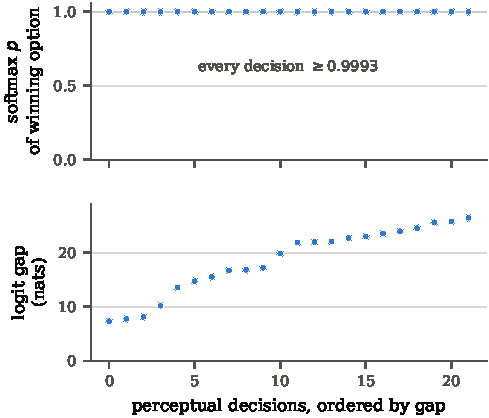
\includegraphics[width=\columnwidth]{figures/saturation.pdf}
\caption{The same 22 decisions and the same forward passes, read two ways.
Top: the softmax probability of the winning option is indistinguishable from
1.0 everywhere. Bottom: the logit gap behind those probabilities spans
7.3--26.4 nats and orders the decisions by difficulty.}
\label{fig:saturation}
\end{figure}

Every one of the 22 decisions reports a winning-option probability of at least
$0.9993$ (Figure~\ref{fig:saturation}, top). Taken at face value the system is
certain about all of them, and no threshold on that number can separate the
item it found hardest from the item it found easiest. On MMBench the
saturation is severe but not total---the minimum is 0.325 and 88\% of items
exceed 0.99---so this figure overstates the effect; what survives at scale is
the consequence, that the probability is $\geq 0.99$ on 52\% of the model's
errors (Section~\ref{sec:mmbench}). The information is not
absent from the model; it is destroyed by the readout. A softmax over two or
three slots maps any gap beyond roughly 7 nats to a probability that rounds to
one. The gaps themselves (Figure~\ref{fig:saturation}, bottom) are well spread
and monotone in our a priori difficulty ordering. The upstream implementation
labels its output \emph{``conditional option score; uncalibrated as decision
confidence''}, which is correct but understates the problem: the quantity is
not a weak confidence signal, it is very nearly a constant. Practitioners who
need a threshold should apply it to the gap in nats.

\subsection{Order sensitivity is small}
\label{sec:order}

Averaged over rotations, the mean logit assigned to each letter slot differs
by 0.2--2.4 nats, with no consistent preference for the first slot. Against
perceptual gaps of 7.3 nats and above, this is an order of magnitude too small
to matter, and indeed the winner changes under rotation in 0 of 22 perceptual
decisions. Order calibration on this workload costs $n$ forward passes and buys
nothing. It is not free elsewhere: in the text-model experiments of
Section~\ref{sec:cascade}, where gaps fall to 0.8--2.3 nats, the same 1--2 nats
of position bias decides the answer outright and the winner flips.
A practical rule follows: rotate and average only when the single-pass gap is
below roughly 3 nats.

\subsection{The gap does not gate normative questions}
\label{sec:families}

\begin{figure}[t]
\centering
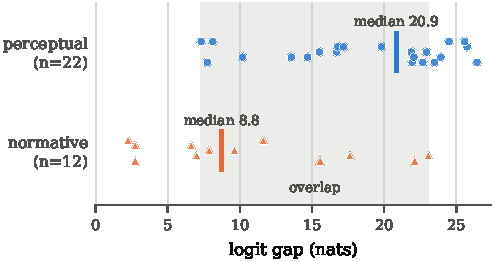
\includegraphics[width=\columnwidth]{figures/families.pdf}
\caption{Logit gaps for 22 perceptual decisions and 12 normative ones under the
same model and readout. The distributions differ (AUC 0.788, $p=0.006$) but
overlap over most of their range; the shaded band marks the overlap.}
\label{fig:families}
\end{figure}

If the gap tracks difficulty within a family, the natural hope is that it also
flags questions the model has no business answering. We tested this on the 12
normative items, which are unanswerable in principle rather than merely hard.

The hope fails (Figure~\ref{fig:families}). The distributions do differ:
median 8.8 nats for normative against 20.9 for perceptual, giving an AUC of
0.788 (Mann--Whitney $U=208$, $z=2.74$, $p=0.006$). But 7 of 12 normative items
fall inside the perceptual range, and the best achievable threshold, 7.3 nats,
retains all 22 perceptual decisions only by admitting 7 of the 12 normative
ones---79\% accuracy for a filter whose entire purpose is to catch the
remainder. Individual cases are worse than the aggregate suggests. The model
asserts that a photograph with a colour cast should enter the correction queue
at 23.1 nats and that publication must be held for consent at 15.6, both
policy questions, at gaps indistinguishable from its report that there is no
dog in the picture (26.4). Only 1 of 12 normative items flips under rotation.

Two of our normative items are arguably entailed by their evidence, which
inflates their gaps and weakens the contrast; we note this rather than remove
them post hoc.

\subsection{Validation at scale on MMBench}
\label{sec:mmbench}

\begin{table}[t]
\centering\small
\caption{Qwen3-VL-4B on MMBench en/dev (4329 items). CircularEval requires the
correct answer under every rotation of the options.}
\label{tab:mmbench}
\begin{tabular}{lrrr}
\toprule
Protocol & Accuracy & ms/item & AUC gap \\
\midrule
VanillaEval  & 87.4\% & 91  & 0.894 \\
CircularEval & 82.2\% & 347 & 0.956 \\
\bottomrule
\end{tabular}
\end{table}

Our own benchmark returned 22/22, so it could not measure whether the gap
\emph{predicts} anything---there were no errors to predict. MMBench supplies
547 of them under VanillaEval.

The gap separates correct from incorrect answers with AUC 0.894 ($z=29.9$),
with a median of 22.4 nats when the model is right against 5.2 when it is
wrong. Thresholding on it yields a genuine abstention policy: at 12 nats the
system answers 75\% of items at 96.8\% accuracy, and at 16 nats 66\% at 98.4\%,
against an 87.4\% base rate. The reported probability supports nothing
comparable---it is at least 0.99 on 88\% of all items and, more to the point,
on 52\% of the errors.

CircularEval costs 5.2 points (87.4\% to 82.2\%) because the winner changes
under rotation on 507 of 4329 items, 11.7\%. Those items are not randomly
distributed: their median gap is 2.7 nats against 22.8 for the order-stable
ones, and the gap predicts stability with AUC 0.980. The rule we proposed in
Section~\ref{sec:order} from a 22-item probe---rotate only below roughly 3
nats---was written before this dataset was downloaded and lands on the
empirical median of the items that actually flip.

The weakest categories are \texttt{spatial\_relationship} (34.5\% under
CircularEval, against a 25\% chance rate) and \texttt{image\_quality}
(57.3\%). The two lowest gaps in our hand-built probe were its spatial-relation
item (8.1 nats) and its white-balance item (7.8). A confidence signal read off
a handful of examples identified the categories that collapse at scale.

\subsection{Hybrid CPU--GPU execution}
\label{sec:cascade}

\begin{table}[t]
\centering\small
\caption{Latency of one decision, by model and placement. CPU figures are
float32; thread counts are the best of a sweep.}
\label{tab:latency}
\begin{tabular}{llrr}
\toprule
Model & Device & Threads & ms/forward \\
\midrule
Qwen3-VL-4B  & RTX 3080 & --- & 110--140 \\
Qwen3-0.6B   & i9-12900F & 20 & 340--450 \\
Qwen3.5-4B   & i9-12900F & 8  & 1359 \\
Qwen3.5-4B   & i9-12900F & 20 & 2392 \\
\bottomrule
\end{tabular}
\end{table}

Because the two devices are idle at different times, we built a two-stage
cascade: the GPU resolves visual predicates over an image, and a CPU model
decides an action from the resulting verdicts without ever seeing pixels. Run
as two threads with a queue between them, the stages overlap---PyTorch releases
the interpreter lock during both CUDA and CPU forwards---and wall-clock time
falls from 3.49\,s to 2.72\,s over four images, a 22\% saving.

The thread sweep in Table~\ref{tab:latency} is a practical result in its own
right. On this hybrid CPU, restricting inference to the 8 performance cores is
$1.9\times$ faster than using 20 threads; scheduling work onto the efficiency
cores actively hurts. Any measurement taken at the default thread count
understates CPU inference on such parts, and our own first cascade measurements
did.

The policy stage itself did not work, and the way it failed is instructive. Our
first design asked one four-option question whose options were not mutually
exclusive---an image can need both colour correction and a consent hold. The
model oscillated between two \emph{correct} answers, which is a defect of the
question, not of the model. Restructuring the stage as independent binary
predicates composed in ordinary Python removed the ambiguity. Even then,
Qwen3-0.6B answered 1 of 4 policy cases correctly and was unstable under
rotation in 3; Qwen3.5-4B answered 3 of 4 and was stable in all 4, but at gaps
of 0.7--2.3 nats, below the threshold at which we would trust any of them. The
larger model also shifts the pipeline from balanced to $12{:}1$ against the CPU
stage, which removes the reason to split the work in the first place.

\section{Discussion}

The perceptual result is strong and the systems result is modest; the two
negative results are what we would want a practitioner to take away.

The first is a readout defect with a one-line fix. Reporting a softmax over
two or three answer slots produces a number that is always approximately one,
and pipelines that threshold on it are thresholding on noise. The gap in nats
is already computed and should be reported instead.

The second is harder to fix and easier to get wrong in production. A semantic
if will answer a question about your organisation's consent policy with the
same apparent conviction it brings to counting cats, and no signal we measured
reliably distinguishes the two. The pattern is therefore safe where the
predicate is perceptual and grounded in the input, and unsafe where the
predicate is normative. Business policy belongs in code. This is also the
lesson of the cascade: the mechanism is called a semantic \emph{if} for a
reason, and composing several binary ifs in a host language is both more
accurate and more debuggable than asking one model to resolve a multi-way
policy.

\paragraph{Limitations.} One model, one prompt template, one language, a
single machine and a single run, without repetition or confidence intervals on
latency. MMBench dev is public and may appear in the model's training data, so
87.4\% is not evidence about generalisation; the claims we defend are about the
confidence signal, which is measured within the same run and does not depend on
the absolute score. Our hand-built probe is small and author-annotated, one of
its labels was demonstrably wrong before correction, and its 22/22 misled us
about the extent of softmax saturation until the larger run corrected it---which
is itself the clearest argument in this paper against trusting a small
author-written benchmark. The normative set has 12 items, two of which are
arguably entailed by their evidence.

\section{Conclusions}

Reading a decision from answer-token logits transfers to vision--language
models without modification and is accurate and fast on grounded perceptual
predicates: 22 of 22 at 110--140\,ms per decision on one consumer GPU, robust
to option order, and correct on counting, absence, false premises and
unanswerable questions. The probability such systems report is not usable as
confidence---it exceeded $0.9993$ on every decision we ran---while the logit
gap behind it is a good within-family difficulty signal. That signal does not
generalise across question families: it fails to separate perceptual questions
from normative ones well enough to gate them, and the model is confidently
wrong about policy. Use semantic ifs for perception, keep policy in code, and
threshold on nats rather than on probabilities.

\section*{Code and data}

Code, benchmark, raw results and this paper's sources are available at
\url{https://github.com/XxSamaxX/siv-semantic-if-vision}. The scoring engine is vendored
from SemIf \cite{semif} under the MIT licence.

\bibliographystyle{plain}
\bibliography{refs}

\end{document}
